\documentclass{article}
\usepackage[utf8]{inputenc}
\usepackage[portuguese]{babel}
\usepackage{graphicx}
\usepackage{booktabs}
\usepackage{amsmath}
\usepackage{natbib}

\title{Relatório da Lista 01 - Análise de Dados}
\author{Laura Nicoletti}
\date{\today}

\begin{document}

\maketitle

\section{Introdução e Dados}
Este relatório utiliza o conjunto de dados \texttt{airquality}, nativo da linguagem R \citep{RCoreTeam}, e os códigos foram formatados utilizando o pacote styler \citep{stylerPacote}. Os dados contêm 153 observações. Na variável Ozone, existem 37 valores faltantes (NAs) que precisaram ser tratados na análise.

Como podemos ver na Tabela \ref{tab:resumo}, os dias medidos em cada mês variam.

\begin{table}[htbp]
\centering
\caption{Resumo dos dados por mês.}
\label{tab:resumo}
\begin{tabular}{lcc}
\toprule
Mês & Média de Ozone & Dias Medidos \\
\midrule
Maio & Valor1 & 31 \\
Junho & Valor2 & 30 \\
Julho & Valor3 & 31 \\
Agosto & Valor4 & 31 \\
Setembro & Valor5 & 30 \\
\bottomrule
\end{tabular}
\end{table}

\section{Análise Gráfica e Cálculos}
A Figura \ref{fig:ozone} ilustra a distribuição dos níveis de ozônio agrupados por mês.

\begin{figure}[htbp]
\centering
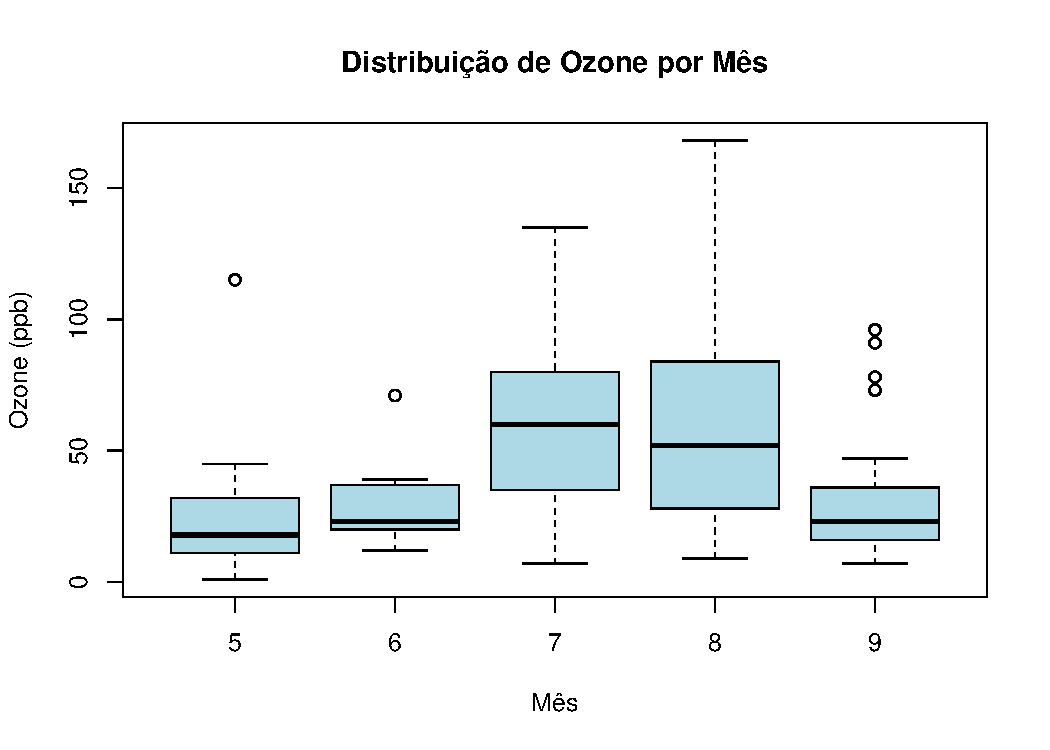
\includegraphics[width=0.8\textwidth]{figura.pdf}
\caption{Distribuição de Ozone por Mês.}
\label{fig:ozone}
\end{figure}

O nosso script \texttt{resumo.sh} realizou o cálculo da média, cuja fórmula pode ser vista na Equação \eqref{eq:media}:

\begin{equation}
\bar{x} = \frac{1}{n} \sum_{i=1}^{n} x_i
\label{eq:media}
\end{equation}

Quando há valores ausentes (NAs) na amostra, o denominador $n$ na equação representa apenas a contagem das observações válidas, ignorando as linhas em branco.

\section*{Declaração de uso de IA}
Neste trabalho, utilizei o assistente de inteligência artificial Gemini para auxiliar na formatação do documento em LaTeX, na compreensão dos comandos do Git Bash e na estruturação dos arquivos. Conferi os resultados testando os scripts no terminal e compilando o documento PDF para garantir que as exigências matemáticas e visuais estavam corretas.

\bibliographystyle{plainnat}
\bibliography{referencias}

\end{document}